\documentclass[aspectratio=169]{beamer}

% because we need to claim weird things
\newtheorem{claim}{Claim}
\newtheorem{defn}{Definition}
%\newtheorem{lemma}{Lemma}
\newtheorem{thm}{Theorem}
\newtheorem{vita}{Vit\ae}
\newtheorem{qotd}{Quote of the Day}

\usepackage{algorithm}
\usepackage{algpseudocode}
\usepackage{listings}
\usepackage{color}
\usepackage{graphics}
\usepackage{ulem}
\bibliographystyle{unsrt}

% background image
\usebackgroundtemplate%
{%
    
\includegraphics[width=\paperwidth,height=\paperheight]{../artifacts/stemulus.pdf}%
}
\setbeamertemplate{caption}[numbered]
\lstset{%
	breaklines=true,
	captionpos=b,
	frame=single,
	keepspaces=true,
	showstringspaces=false
}

% page numbers
\addtobeamertemplate{navigation symbols}{}{%
    \usebeamerfont{footline}%
    \usebeamercolor[fg]{footline}%
    \hspace{1em}%
    \insertframenumber/\inserttotalframenumber
}

% presentation header
\usetheme{Warsaw}
\title{IPv6 For Web Developers}
\author{Dylan Lane McDonald}
\institute{CNM STEMulus Center\\Web Development with PHP}
\date{\today}

\begin{document}
\lstset{language=Java}
\begin{frame}
\titlepage
\end{frame}

\begin{frame}
\frametitle{Outline}
\tableofcontents
\end{frame}

\section{IPv4 vs. IPv6}
\begin{frame}
\frametitle{Executive Summary}
\begin{itemize}
	\item The current pool of IPv4 addresses is nearly exhausted
	\pause
	\item IPv4 was originally setup experimentally and just ``caught on''
	\pause
	\item IPv6 presents a long term, sustainable solution to the problem
	\pause
	\item IPv6 is easy to deploy and enjoys wide ``out of the box'' operating system support
	\pause
	\item IPv6's main barriers to wide deployment are:
	\begin{itemize}
		\pause
		\item \textbf{ISPs}: staying on older IPv4 implementations
		\pause
		\item \textbf{End Users}: with aging, IPv6 incompatible modems \& routers
		\pause
		\item \textbf{Software Developers}: writing software that are merely IPv4 aware
	\end{itemize}
\end{itemize}
\end{frame}

\subsection{Review of how IPv4 works}
\begin{frame}
\frametitle{OSI Model}
The \textbf{OSI Model} is a layered approach of all network traffic.
\begin{table}
\begin{tabular}{|l|l|l|}
\hline
\textbf{\#} & \textbf{Layer} & \textbf{Example}\\
\hline
7 & Application & HTTP, SMTP, SSH, DHCP\\
\hline
6 & Presentation & SSL/TLS, UTF-8, JSON\\
\hline
5 & Session & PPTP, RPC, SMB\\
\hline
4 & Transport & TCP, UDP\\
\hline
3 & Network & IP, IPSec, ICMP\\
\hline
2 & Data Link & PPP, AppleTalk, Ethernet, Wi-Fi\\
\hline
1 & Physical & DSL, Cable, PSTN\\
\hline
\end{tabular}
\caption{OSI Model}
\label{tbl:osi}
\end{table}
Table \ref{tbl:osi} lists the layers and examples. Most web development is at layers 6 \& 7. Today's discussion will also focus on layer 3.
\end{frame}

\begin{frame}
\frametitle{DHCP \& SLAAC}
IPv4 is primarily ``autoconfigured'' using \textbf{D}ynamic \textbf{H}ost \textbf{C}onfiguration \textbf{P}rotocol (DHCP). DHCP was originally designed as an extension to BOOTP, a network method of booting a diskless workstation from the network.

\pause
\mbox{}\\
IPv6 has two methods of configuring: DHCPv6, which is IPv6 DHCP and \textbf{S}tateless \textbf{A}ddress \textbf{A}uto\textbf{c}onfiguration (SLAAC). SLAAC essentially asks everyone around you for the gateway and network part of the IPv6 address. The large advantage of this is that there's no single point of failure (the DHCP server).
\end{frame}

\begin{frame}
\frametitle{The IPv4 Address}
The most familiar form of an IPv4 address is \emph{dotted quad notation}. This notation denotes the constituent bits of the IPv4 address in a human readable format.
\pause
\[
\underbrace{\underbrace{\underbrace{198}_{11000110}}_{\textnormal{first byte}}.\underbrace{\underbrace{251}_{11111011}}_{\textnormal{second byte}}.\underbrace{\underbrace{70}_{01000110}}_{\textnormal{third byte}}.\underbrace{\underbrace{220}_{11011100}}_{\textnormal{fourth byte}}}_{32 \textnormal{ bits } = \textnormal{ } 4 \textnormal{ bytes}}
\]
\pause
With 32 bits, the theoretical limit on IPv4 is $2^{32} \approx $ 4.2 billion IPv4 addresses. With the world population currently at 7.2 billion, that is 1 IPv4 address per 1.67 people. \cite{census}
\end{frame}

\begin{frame}
\frametitle{The IPv6 Address}
An IPv6 address is written in hexadecimal notation. For instance, \texttt{2001:470:4b:1f4:dee7:d16:9ec0:de72}. While this may look intimidating, hexadecimal was chosen because it can represent many more bytes in a smaller space.

\pause
\[
\underbrace{\underbrace{2001}_{\textnormal{first 2 bytes}}:\underbrace{0470}_{\textnormal{second 2 bytes}}:\dots:\underbrace{\textnormal{de72}}_{\textnormal{eighth 2 bytes}}}_{128\textnormal{ bits }=\textnormal{ 16 bytes}}
\]

\pause
IPv6 addressing is not fundamentally different than IPv4 addressing is. Other than the obvious difference in the size \& representation of the address space, the concepts remain exactly the same.
\end{frame}

\begin{frame}
\frametitle{Subnetting}
Each IPv$X$ address consists of two sections: the network and host section. The division of the network and host sections are determined by the individual ISPs and systems administrators.

\mbox{}\\
The canonical way of addressing and making the network/host boundary known is to use CIDR\footnote{\textbf{C}lassless \textbf{I}nter-\textbf{D}omain \textbf{R}outing} notation. This indicates the number of bits for the network section of the IP address. Given the following 2 IPs:

\texttt{198.251.70.220/28\\
2001:470:4b:1f4:dee7:d16:9ec0:de72/96}

\mbox{}\\
The IPv4 has 28 bits for the network section and 4 bits for the host section. Similarly, the IPv6 has 96 bits for the network section and 32 bits for the host section.
\end{frame}

\begin{frame}
\frametitle{Common IPv4 \& IPv6 subnets}
The common IPv4 subnets are:
\begin{itemize}
	\item /8: ``Class A'': $2^{24} = 16,777,216$ addresses
	\item /16: ``Class B'': $2^{16} = 65,536$ addresses
	\item /24: ``Class C'': $2^{8} = 256$ addresses
\end{itemize}
A /8 is the largest unit distributed from IANA to the RIRs. A /24 is what the vast majority of home routers work with.

\pause
\mbox{}\\
The common IPv6 subnets are:
\begin{itemize}
	\item /48: large site deployment $2^{80} \approx 1.209 \times 10^{24}$ addresses
	\item /64: end user deployment $2^{64} \approx 1.845 \times 10^{19}$ addresses
	\item /96: small end user deployment $2^{32} = 4,294,967,296$ addresses
\end{itemize}
Notice the ``smallest'' IPv6 subnet is enough to fully accomodate all possible IPv4 addresses.
\end{frame}

\subsection{IPv4 Exhaustion Problem}
\begin{frame}
\frametitle{IPv4 Exhaustion Problem}
Isn't 1 IPv4 address per 1.67 people enough?

\pause
\mbox{}\\
\textbf{No!} Every device you have needs an IP address! Your:
\begin{enumerate}
	\item Laptop
	\pause
	\item Desktop
	\pause
	\item Phone
	\pause
	\item Tablet
	\pause
	\item iPod
	\pause
	\item PlayStation
	\pause
	\item Roku
	\pause
\end{enumerate}
Need I go on!?
\end{frame}

\begin{frame}
\frametitle{Regional IP Address Control}
\begin{figure}
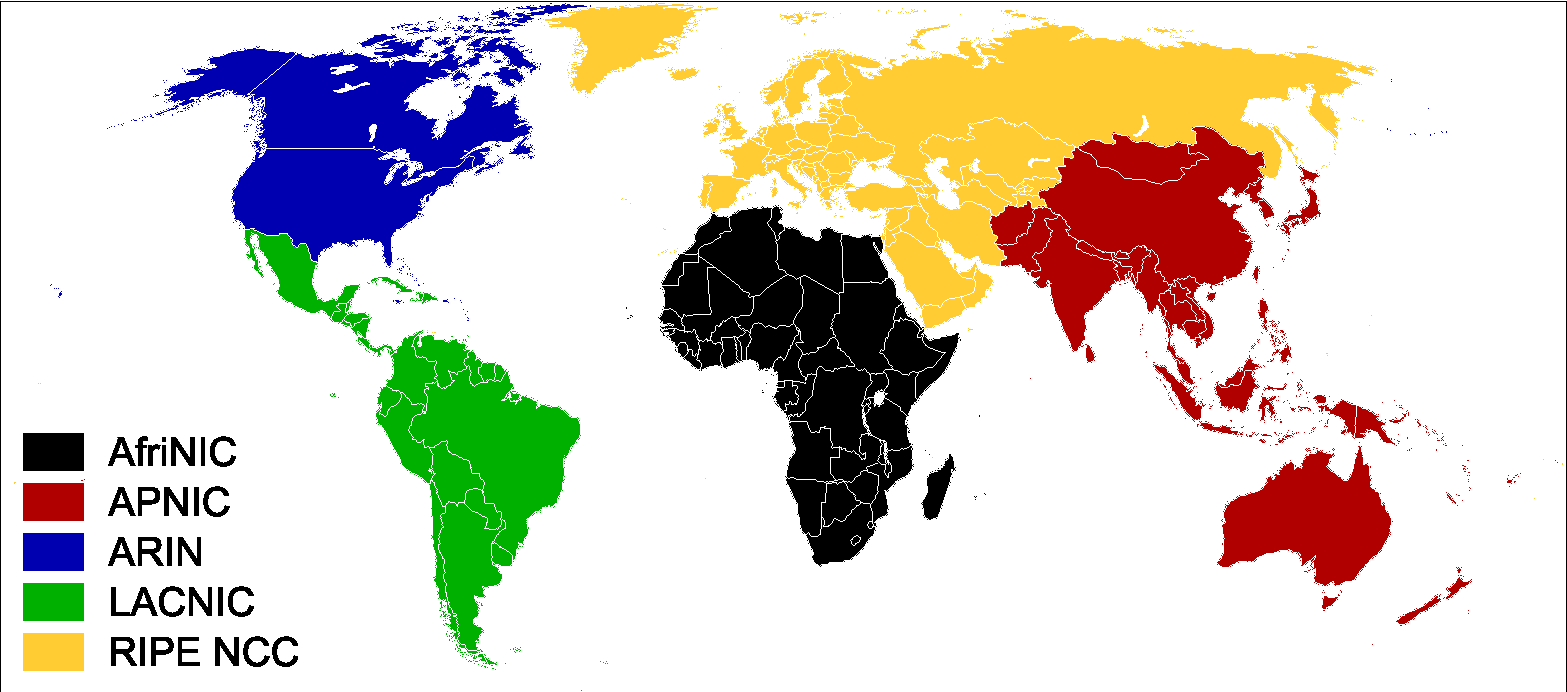
\includegraphics[scale=0.44]{../artifacts/regional-registries.pdf}
\caption{Regional Registries}
\label{fig:regional}
\end{figure}
\end{frame}

\begin{frame}
\frametitle{Regional Statistics}
Currently, the regional authorities are reporting the following number of IPv4 addresses: \cite{he-stats}
% April 2014 numbers:
% 52666547
% 13317961
% 21312980
% 12939955
% 13889015
\begin{table}
\begin{tabular}{|l|l|l|}
\hline
\textbf{Region} & \textbf{Remaining IPv4s} & \textbf{\% Change Since April 2014}\\
\hline
Africa & 28,245,012 & -51.5238 \%\\
\hline
Asia/Pacific & 9,998,932 & -42.4475 \%\\
\hline
North America & 0 & -100.00 \%\\
\hline
Latin America & 1,622,440 & -93.8697 \%\\
\hline
Europe & 15,497,486 & +2.0675 \%\\
\hline
\end{tabular}
\caption{Remaining IPv4s by Region}
\label{tbl:remaining}
\end{table}
Asia/Pacific exhausted in April 2011. Europe exhausted in September 2012. North America exhausted in April 2014. \cite{arin} Latin America exhausted in June 2014. \cite{lacnic}
\end{frame}

\begin{frame}
\frametitle{IPv4 Doomsday!}
OK, so all the regional authorities are out of IPv4 addresses. What then?
\begin{itemize}
	\pause
	\item The owners of the IPv4 addresses will still retain ownership of those addresses.
	\pause
	\item The existing IPv4 infrastructure will live on, but with no room to grow or expand.
	\pause
	\item TCP/IP was designed with unobstructed, end-to-end communication in mind.
		\begin{itemize}
			\pause
			\item ISP quality NAT, while it has delayed the inevitable slightly, breaks this end-to-end communication.
			\pause
			\item This problem has been exacerbated by the explosion in connected mobile devices.
		\end{itemize}
\end{itemize}
The only true long term solution is IPv6.
\end{frame}

\subsection{How IPv6 improves IPv4}
\begin{frame}
\frametitle{IPv6 Improvements}
The most obvious improvement in IPv6 is mind boggling number of addresses. $2^{128} \approx 3.40282 \times 10^{38} \approx$ 340 trillion trillion trillion. That's still enough IP addresses to grant every grain of sand on the earth and every single cell on every single human an entire IP space the size of IPv4 and still have IP addresses to spare!

\pause
\mbox{}\\
In addition to the mammoth IP address space, IPv6 enjoys the following features:
\begin{itemize}
	\item Built in security (IPSec)
	\pause
	\item More efficient routing
	\pause
	\item Easier auto-configuration
\end{itemize}
\end{frame}

\section{How to Deploy IPv6 with very Little Effort}

\subsection{End Point Approaches}
\begin{frame}
\frametitle{End Point Approaches}
There are two approaches to deploying IPv6 on a home or business network:
\pause
\begin{enumerate}
	\item \textbf{Dual Stack}: Running IPv4 and IPv6 simultaneously, this is the ideal situation. One can access IPv6 enabled sites and services in an easy and efficient manner while maintaining IPv4 access to the numerous sites that haven't migrated to IPv6.
	\pause
	\item \textbf{Tunnel}: Deploying IPv6 inside of IPv4, this is an alternative to those who cannot use a dual stack approach. The systems administrator sets up a tunnel with an IPv6 provider and grants IPv6-enabled access to the local network.
\end{enumerate}

\pause
Dual stack is by far the most efficient method and is easiest to setup. Where possible, dual stack is preferred.
\end{frame}

\subsubsection{Dual Stack}
\begin{frame}
\frametitle{Dual Stack}
In order to have a dual stack network, one needs:
\begin{enumerate}
	\item \textbf{ISP}: An ISP providing IPv6 service
	\pause
	\item \textbf{Modem/Router}: Modem and/or router that supports IPv6
	\pause
\end{enumerate}
%Most modems/router manufactured in the past 2 years are IPv6 compatible. So, older equipment may need to be upgraded.
\begin{table}
\begin{tabular}{|l|l|}
\hline
\textbf{ISP} & \textbf{IPv6?}\\
\hline
AT\&T DSL & yes\\
\hline
AT\&T Wireless & no\\
\hline
CenturyLink & yes\\
\hline
Comcast & yes\\
\hline
Sprint & no\\
\hline
T-Mobile & yes\\
\hline
Verizon Wireless & yes\\
\hline
\end{tabular}
\caption{IPv6 Compatible ISPs}
\label{tbl:isps}
\end{table}
\end{frame}
\subsubsection{Tunnels}
\begin{frame}
\frametitle{Tunnels}
A \textbf{tunnel} is a service provided by a \textbf{broker}, an upstream ISP that has IPv6 access. Packets are sent from the endpoint to through the tunnel via IPv4, thus negating the necessity for native IPv6 at the end point. Many IPv6 enabled routers can be configured to use a tunnel out-of-the-box.

\pause
\mbox{}\\
Tunnelbroker \& Sixx are the most popular brokers and are integrated into most end user's router configuration pages. Once the tunnel is created and configured, IPv6 will be enabled on the local network.
\end{frame}

\subsection{Server Approaches}
\begin{frame}
\frametitle{Server Approaches}
Recently, I changed my domain to a dual stack server. The exact steps taken were:
\begin{enumerate}
	\item Ask web host for an IPv6 subnet (5 minutes).
	\pause
	\item Configure server's ethernet card to use an IPv6 address (10 minutes).
	\pause
	\item Reconfigure Apache (0 minutes).
	\pause
	\item Create forward DNS records (10 minutes).
	\pause
	\item Ask web host to create reverse DNS records (5 minutes).
	\pause
\end{enumerate}
That's right! Apache worked with IPv6 immediately! Ever since then, the dual stack web server has been chugging along transparently irrespective as to whether IPv4 or IPv6 clients are connecting.
\end{frame}

\section{IPv4 to IPv6 Migration of Web Applications}
\begin{frame}
\frametitle{Storing IP addresses}
As just discussed, IP addresses are just numbers. To convert the ASCII (string) format, PHP has the \texttt{ip2long()} function for IPv4 addresses. The traditional wisdom was to use this function and store the IPv4 address as an \texttt{INTEGER UNSIGNED} in mySQL.

\pause
\mbox{}\\
The new way is to store IPv$X$ addresses as raw binary data and store it in mySQL as \texttt{VARBINARY(16)} to effectively accommodate both IPv4 and IPv6 addresses. In PHP, use the \href{http://www.php.net/manual/en/function.inet-ntop.php}{\texttt{inet\_ntop()}} to retrieve IPs and \href{http://www.php.net/manual/en/function.inet-pton.php}{\texttt{inet\_pton()}} to store IPs. This will create an efficient solution that is both IPv4 and IPv6 compatible.
\end{frame}

\begin{frame}
\frametitle{IPv6 Application ``Y2K'' Problem}
The real impact on web developers, and developers in general, is IPv6-enabling applications. The previous discussion about storing IPv6 addresses is only the beginning. After you're enabled with a dual-stack web server, code modifications abound\dots
\begin{itemize}
	\item Changing mySQL table definitions
	\item Refactoring IP-based access lists to support IPv6
	\item Enhancing logic that deals with geolocation of IPs
	\item IPv6 enabling code that depends on DNS queries
	\item \textbf{Regression testing} a new IPv6 application
\end{itemize}
IPv4 will be around for some years to come. IPv6 will need to cooperate with IPv4 while the world is in transition. This cannot happen without great developers.
\end{frame}

\begin{frame}
\frametitle{Works Cited}
\bibliography{ipv6}
\end{frame}
\end{document}
